\chapter{Аппаратура для проведения исследований} \label{chapt2}

\section{Прибор Дэпрон}

Прибор Дэпрон разрабатывался как исследовательский инструмент для решения широкого круга научных задач. Основной задачей прибора является измерение мощности дозы и потоков ионизирующих излучений. Дополнительными задачами выделены регистрация нейтронов тепловых энергий и высокоэнергетичных частиц. Такое сочетание решаемых задач, для прибора относительно небольшого веса,  является уникальным и позволяет надеяться на получение достаточно подробной информации о радиационной обстановке на борту КА. 

\subsection{Устройство прибора}

В состав прибора ДЭПРОН входят два узла с полупроводниковыми детекторами и два узла с газоразрядными гелиевыми счетчиками нейтронов. Также в состав прибора входят узлы усиления и формирования сигналов от полупроводниковых и нейтронных детекторов и узел цифровой обработки сигналов.


Поглощенная доза регистрируется узлами с полупроводниковыми детекторами. Для получения информации о величине поглощенной дозы используется принцип регистрации величины заряда в объеме полупроводника, пропорционального энерговыделению в данном объеме. 

\begin{equation}\label{eq:benghin_doze}
D = \frac{E}{m} = \dfrac{w_i \cdot\dfrac{q}{e}}{m}
\end{equation}
где \begin{description}
	\item[$ D $] поглощенная доза
	\item[$ E $] энергия поглощенная в чувствительном объеме
	\item[$ m $] масса чувствительной зоны детектора
	\item[$ w_i $] энергия формирования np пары
	\item[$ e $] заряд электрона
	\item[$ q $] электрический заряд образованный в чувствительном объеме
\end{description}
Оба полупроводниковых детектора и скомпонованы в кассету и расположены в относительной близости друг от друга. Схема построения прибора с параллельным расположением двух полупроводниковых детекторов была использована для получения информации о ЛПЭ частиц, прошедших одновременно оба детектора. Спектр ЛПЭ зарегистрированных частиц позволяет вычислить эквивалентную дозу, используя постулированный в НРБ коэффициент качества ионизирующего излучения. Для перехода от поглощенной дозы в кремнии к эквивалентной дозе потребуется пересчет зарегистрированного спектра ЛПЭ в спектр ЛПЭ в воде, который произвадится умножением на коэффициент $ 1,21 $.
 Функциональная схема прибора ДЭПРОН показана на рисунке \ref{fig:Depron_blocksch}.
 
\begin{figure}
\centering
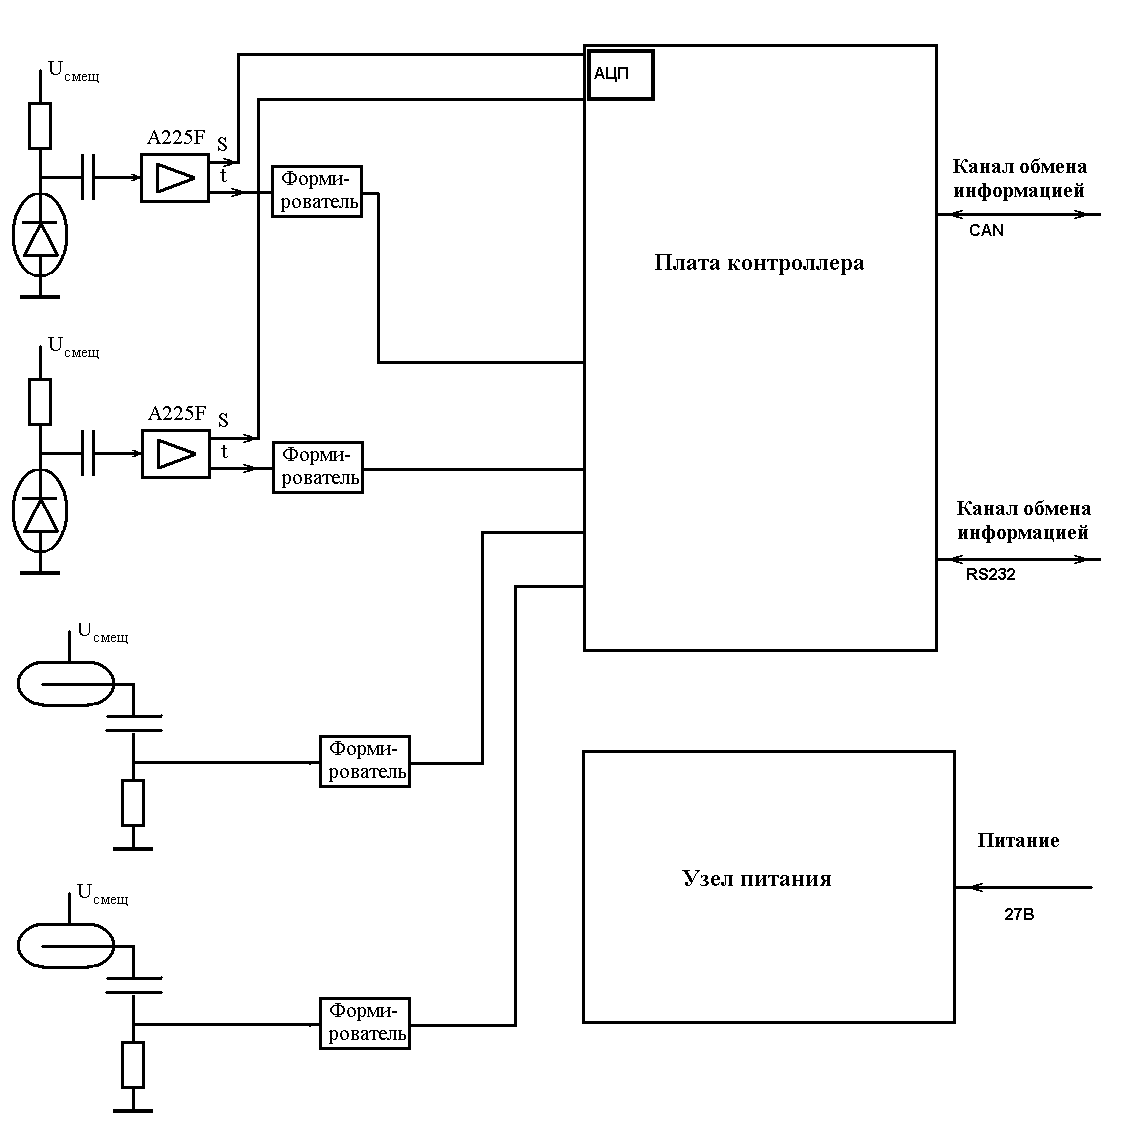
\includegraphics[width=0.8\linewidth]{images/Depron_blocksch}
\caption{Блок-схема прибора ДЭПРОН}
\label{fig:Depron_blocksch}
\end{figure}


%\newpage
%============================================================================================================================
\section{Конструктивные особенности прибора}

Прибор состоит из одного блока, габаритный чертеж которого представлен в Приложении 1. Габаритные размеры прибора: длина  280 мм, ширина 160 мм, высота 78 мм. Масса прибора - 3 кг. Корпус прибора составлен из шести пластин Д16т -- листового дюралюминия, толщиной 4,5 мм, обработанного на станке ЧПУ. В каждой пластине фрезерованы повторяющиеся выборки треугольной формы до толщины 2 мм. Выборки расположены таким образом, чтобы сформировать «ребра» жесткости в стенках прибора, как видно на рисунке \ref{fig:viborki}. С лицевой стороны пластины корпуса оксидированы, с целью получения электропроводной поверхности всего прибора.

\begin{figure}
\centering
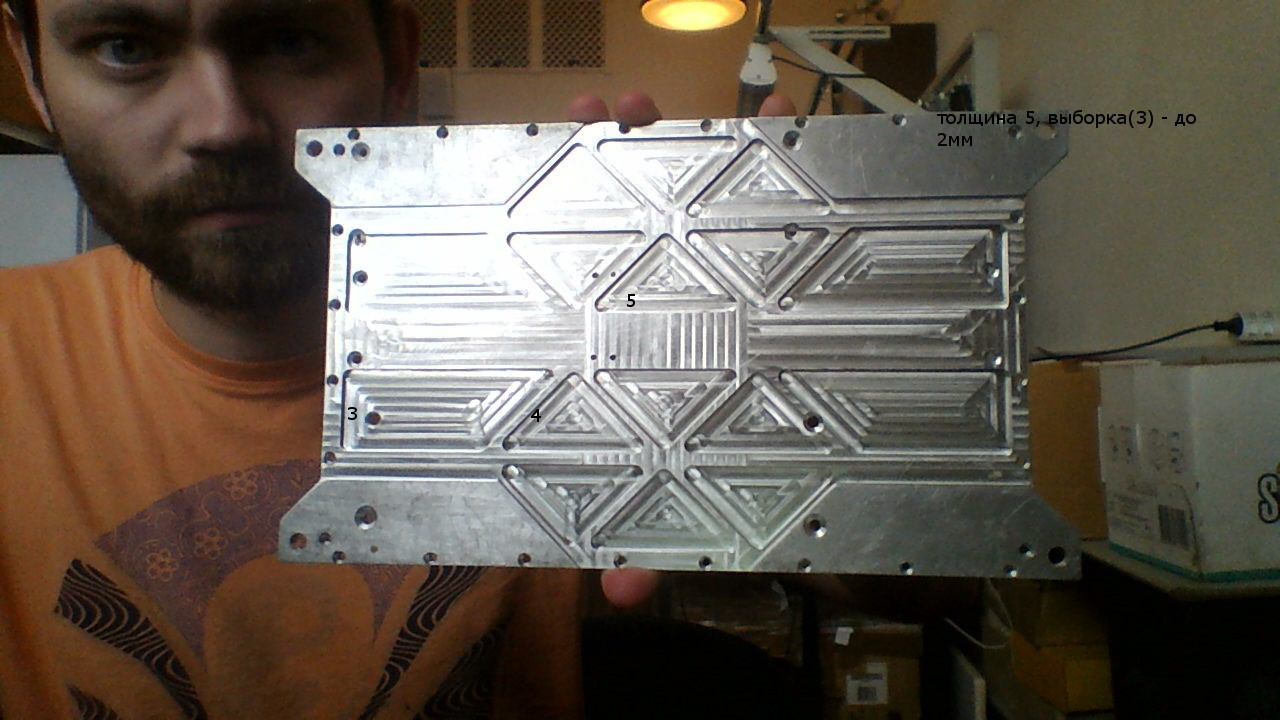
\includegraphics[width=0.7\linewidth]{images/viborki}
\caption{ Вариант размещения выборок в днище прибора ДЭПРОН.}
\medskip
{\small В последствии данный вариант переработан исходя из конструктивных соображений крепления модулей электроники и улучшения теплосброса источников питания, через термоконтакт с бортом КА. }
\label{fig:viborki}
\end{figure}


На лицевом торце прибора распложены два разъема СНП-333, используемых для передачи данных в БИ аппаратуры спутника (разъем Х1) и для передачи питания в прибор ДЭПРОН от бортовой аппаратуры спутника (разъем Х2). Также на лицевой панели находятся два разъема РС-7 предназначенные для передачи информации по каналу RS232 от прибора ИМИСС-1 (разъем Х5) и сквозной передачи питания от бортовой аппаратуры к прибору ИМИСС-1 (разъем Х4). Во всех перечисленных разъемах предусмотрен контроль стыковки разъемов с помощью короткозамкнутых линий, а также дублирование информационных и токонесущих линий.


Дополнительно на лицевую панель прибора вынесен технологический разъем РС 19 ХТ3, используемый для проверки функционирования прибора в лабораторных условиях методом подачи на детекторные узлы калиброванных сигналов с генератора, а также для контроля внутренних рабочих напряжений. Проверка работоспособности прибора и подача сигналов с генератора осуществляется с помощью  блока КПА, имеющему четыре экранированных канала для передачи низкоамплитудных сигналов и два светодиодных индикатора для контроля наличия рабочих напряжений  $ +5  $В и$  +12 $ В в приборе ДЭПРОН.  В штатном режиме работы данный разъем не подключен и закрыт заглушкой. Схема распределения линий в разъемах представлена в Приложении 2.

Платы электроники блоков усиления и формирования аналоговых сигналов располагаются в трех тонкостенных алюминиевых кассетах и выполнены в формате 11-ти контактных печатных плат размерами 34х50мм (\ref{fig:Depron_inside}). Данный формат печатных плат распространен в производстве научной аппаратуры изготовления НИИЯФ МГУ и с успехом применяется для космической аппаратуры уже на протяжении нескольких десятков лет. Применение данного стандарта позволяет соблюсти принцип модульности построения приборов, используя отработанные в космических условиях надежные схемы, компонуя из них тракты с параметрами, заданными потребностями текущих экспериментальных задач. 

\begin{figure}
\centering
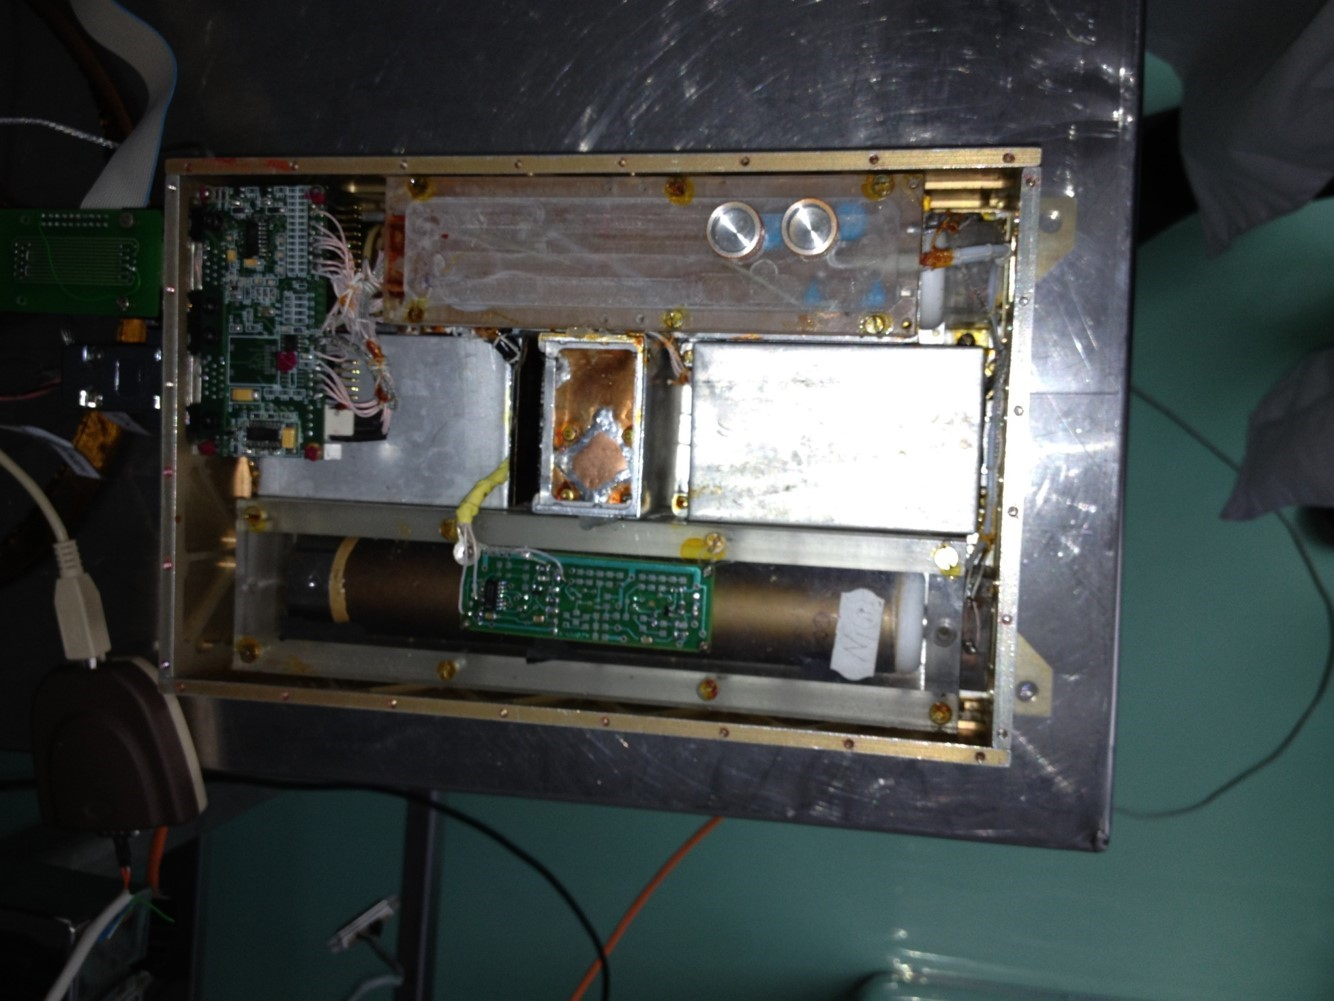
\includegraphics[width=0.7\linewidth]{images/Depron_inside}
\caption{Внутренняя компоновка модулей прибора ДЭПРОН. Вид сверху со снятой крышкой прибора.}
\label{fig:Depron_inside}
\end{figure}


В средней части рисунка последовательно располагаются три корпусных кассеты с платами электроники: левая и правая кассеты содержат платы формирователей триггерных сигналов от детекторов, центральная кассета ориентирована перпендикулярно и содержит две платы полупроводниковых детекторов и ЗЧУ, а также платы дополнительного усиления.

В нижней части рисунка находится нейтронный счетчик СИ13Н (циллиндр), экранированный 1 см оргстекла

\section{Детекторы}

Дозиметр заряженных частиц выполнен на кремниевых ионно-имплантированных Д1 пролетных детекторах, работающих в режиме регистрации амплитуд импульсов. Детекторы изготовлены по специальному заказу НИИЯФ МГУ в ООО «Детектор-СИ» в соответствии с АБЛК.418219.402ТУ. Данные детекторы предназначены для спектрометрии и радиометрии заряженных частиц в составе предназначенной для этих целей аппаратуры. Чувствительный элемент детектора изготовлен из высокоомного кремния n--типа по технологии ионной имплантации. Рекомендуемая схема включения детектора приведена на рисунке \ref{fig:detector_sch}. 


\begin{figure}[h]
	\centering
	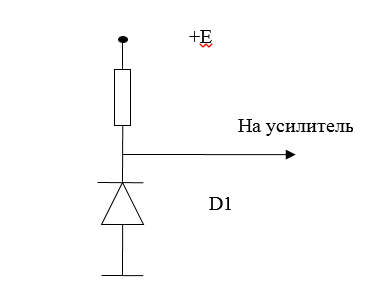
\includegraphics[width=0.5\linewidth]{images/detector_sch}
	\caption{Схема включения детектора.}
	\medskip
	\small
	\begin{description}
		\item[+Еп] источник напряжения;
		\item[Rсм] сопротивление смещения;
		\item[D1] Детектор.
	\end{description}			
	\label{fig:detector_sch}
\end{figure}
	


Детекторы могут эксплуатироваться при атмосферном давлении или в вакууме до 10\textsuperscript{-6} мм.рт.ст., таким образом подходят для расмещения в не герметичном корпусе прибора ДЭПРОН. Подробные значения параметров детекторов приведены в таблице \ref{tab:detectors}.

\begin{table} 

	\begin{tabular}{p{10cm}|cc}
		Наименование параметра&Фактические параметры\\ \hline
		Рабочее напряжение, В&90&\\ Обратный ток, нА&4\\
		Энергетический эквивалент шума, кэВ&5\\
		Постоянная времени квазигауссова формирования импульса, мкс&2\\
		Предельно допустимое напряжение, В&130\\
		\multicolumn{2}{l}{Примечания: Аттестация производилась при 26 C.}\\
		
	\end{tabular} 
	\caption{Полупроводниковые детекторы прибора ДЭПРОН (по материалам ТУ)}
		\label{tab:detectors}
\end{table}



\subsection{Телескоп детекторов}
В приборе Дэпрон  используются два полупроводниковых детектора. Детекторы образуют телескоп, то есть расположены параллельно на определенном расстоянии, что обеспечивает возможность регистрировать спектр ионизационных потерь.
Дополнительно использование двух детекторов позволяет повысить уровень надежности всего регистрирующего тракта.

Схематично относительное расположение детекторов показано на рисунке~\ref{fig:telescope}.  Расстояние между детекторами выбрано 18 мм, таким образом что телесный угол полета частиц, проходящих через оба детектора оказывается около 30 градусов. 


%\begin{tikzpicture}
%\draw[dashed,color=gray] (0,0) arc (-90:90:0.5 and 1.5);% right half of the left ellipse
%\draw[semithick] (0,0) -- (4,1);% bottom line
%\draw[semithick] (0,3) -- (4,2);% top line
%\draw[semithick] (0,0) arc (270:90:0.5 and 1.5);% left half of the left ellipse
%\draw[semithick] (4,1.5) ellipse (0.166 and 0.5);% right ellipse
%\draw (-1,1.5) node {$\varnothing d_1$};
%\draw (3.3,1.5) node {$\varnothing d_2$};
%\draw[|-,semithick] (0,-0.5) -- (4,-0.5);
%\draw[|->,semithick] (4,-0.5) -- (4.5,-0.5);
%\draw (0,-1) node {$x=0$};
%\draw (4,-1) node {$x=l$};
%\end{tikzpicture}



\begin{figure}	
	\centering
	\begin{tikzpicture}[scale=2, transform shape]
	\pic [fill=magenta, text=blue, draw=blue] at (5,0) {annotated cuboid={width=10, height=0.3, depth=10, units=мм}};
	\pic [fill=green, text=green!50!black, draw=green!25!black] at (5,-1.8) {annotated cuboid={width=10, height=0.3, depth=10, units=мм}};
	
	\draw[|->,semithick] (7,-1.8) -- (7,0);
	\draw (8,-1.8) node {$z=0$};
	\draw (8,0) node {$z=18$};
	%	\pic at (1,-3) {annotated cuboid={width=150, height=200, depth=250, scale=.01, units=m}};
	%	\pic [fill=cyan, text=blue!75!cyan, draw=blue!75!cyan] at (-3,-2) {annotated cuboid={width=15, height=18, depth=13.5, units=}};
	\end{tikzpicture}
	\caption{Телескоп детекторов прибора ДЭПРОН, масштаб 1:2}
	\label{fig:telescope}
\end{figure}

\subsubsection{Расчет геометрического фактора телескопа}
В соответствии с работой :[Analytical derivation of the
geometric factor of a
particle detector having
circular or rectangular
geometry
G R Thomas and D M Willis
SRC, Radio and Space Research Station, Ditton Park,
Slough, SL3 9JX
MS received 12 October 1971, in revised form 18 November
1971 ] общий геометрический фактор можно вычислить исходя из соображений затенения одного детектора вторым, что для геометриии с прямоугольными детекторами дает:

\[ G = Z^2 \int_{-X_1}^{X_1} \int_{-Y_1}^{Y_1} 
			\int_{-X_2}^{X_2} \int_{-Y_2}^{Y_2}
			\frac{dx_1dy_1dx_2dy_2}{\left\lbrace Z^2 + (x_2-x_1)^2 + (y_2-y_1)^2\right\rbrace^2 }\]

Численный расчет в пакете Mathcad ( рисунок \ref{fig:mathcadGeomfactor}) дает в результате для нашего случая геометрический фактор 0.145,  так как геометрический фактор отдельного детектора равен $ 4\pi $ и мы имеем два идентичных детектора, поэтому удваиваем результат интегрирования. Поправочный коэффициент для энерговыделения в телескопе детекторов 0,043, он рассчитан по соотношению \ref{eq:lpe_koef}, где $ S_0 $ площадь чувствительной поверхности.
\begin{equation}\label{eq:lpe_koef}
 \xi = \frac{Z}{2 \pi S_0 } \cdot \int_{-X_1}^{X_1} \int_{-Y_1}^{Y_1} 
\int_{-X_2}^{X_2} \int_{-Y_2}^{Y_2}
\frac{dx_1dy_1dx_2dy_2}{\left\lbrace Z^2 + (x_2-x_1)^2 + (y_2-y_1)^2\right\rbrace^2 }^{\frac{3}{2}}
\end{equation}




\begin{figure}[h!]
\centering
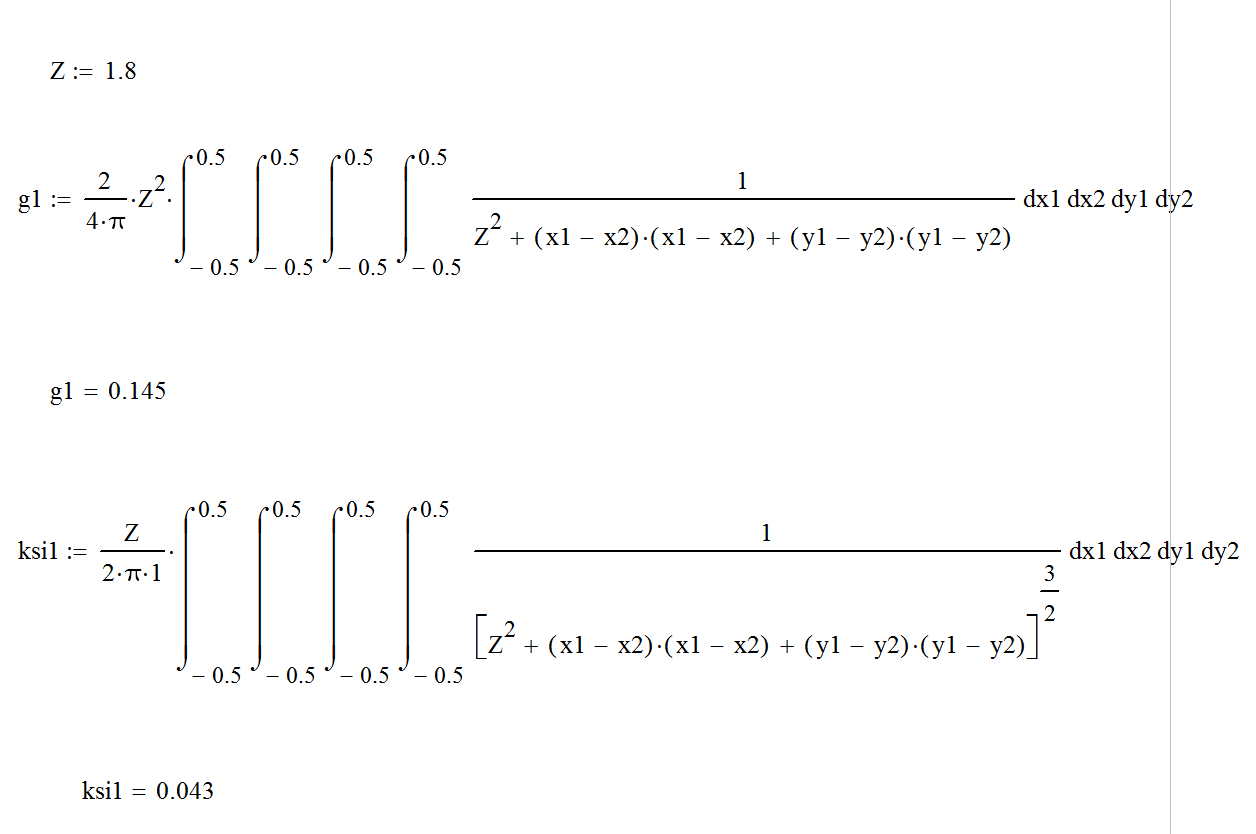
\includegraphics[width=0.7\linewidth]{images/mathcadGeomfactor1}
\caption{ Расчет геометрического фактора телескопа в системе Mathcad}
\label{fig:mathcadGeomfactor}
\end{figure}

%\begin{figure}
%\centering
%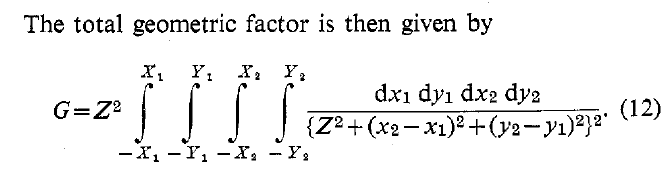
\includegraphics[width=0.7\linewidth]{images/totalgeomfactorintegral}
%\caption{}
%\label{fig:totalgeomfactorintegral}
%\end{figure}

%\begin{figure}
%\centering
%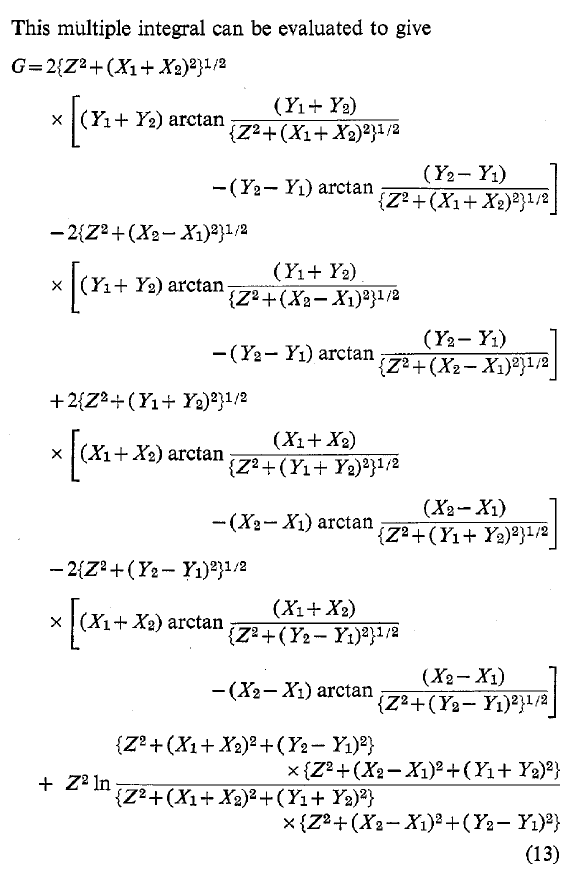
\includegraphics[width=0.7\linewidth]{images/totalgeomfactorsolved}
%\caption{}
%\label{fig:totalgeomfactorsolved}
%\end{figure}
%\begin{figure}
%\centering
%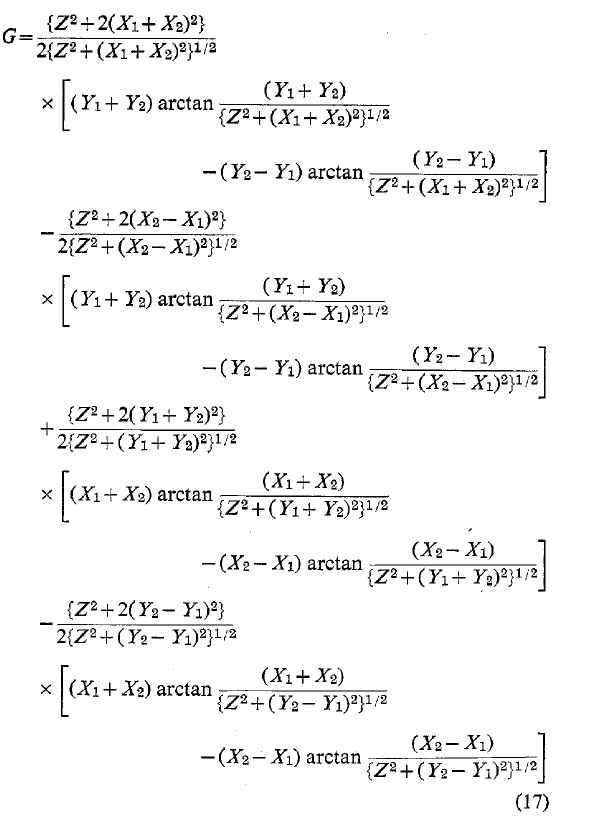
\includegraphics[width=0.7\linewidth]{images/totalgeomfactorsolved2}
%\caption[для интенсивности]{}
%\caption{}
%\label{fig:totalgeomfactorsolved2}
%\end{figure}



\subsection{Нейтронные детекторы}

Детектор нейтронов выполнен на счётчике медленных нейтронов «СИ-13Н», представляющем собой газоразрядный  счетчик, работающий в режиме коронного разряда. Для обеспечения надежности используются 2 счетчика. Второй детектор нейтронов окружен замедляющей оболочной из поликарбоната, что позволило расширить энергетический диапазон регистрируемых нейтронов. При прохождении нейтрона через газ Не-3, наполняющий счетчик, происходит ядерная реакция:
\[ n+^3\!He = p+T+764 \textrm{ КэВ}\]

Продукты реакции вызывают ионизацию газа в счётчике, что приводит к образованию газового разряда и появлению электрического импульса на электроде счетчика. Импульс поступает на вход усилителя-формирователя и, затем, поступает на регистр прерываний процессора, где используется для подсчета числа зарегистрированных нейтронов.
\cite{Shavrin2002}


%\newpage
%============================================================================================================================
\section{Аналоговая обработка сигналов}

Платы полупроводниковых детекторов и предусилителей (внутренний номер SSD006) изготовлены методом фотолитографии в стандартном формате 34х50, использование современных миниатюрных электронных компонент позволило совместить блоки предусиления и детектирования на одной плате и закрыть единым экраном от электромагнитных помех.

Сигнал с полупроводникового детектора поступает на зарядовочувствительный предусилителя A225F, фирмы AMPTEC, специализирующейся на производстве компонент для космической промышленности. 

\todo{Рисунок A225F}

На выходах предусилителя формируются два сигнала. Один (S-сигнал) - имеет амплитуду пропорциональную заряду, образовавшемуся в детекторе и длительность порядка 5 -- 10 мксек. Этот сигнал поступает на амплитудно-цифровой преобразователь (АЦП). Второй сигнал предусилителя A225F (t-сигнал) имеет короткое, менее 0.5 мксек, время задержки от момента прихода сигнала с детектора до максимума амплитуды и используется для запуска процесса цифровой обработки пришедшего импульса. Этот (t-сигнал) сигнал поступает на вход усилителя и, после усиления, поступает на регистр прерываний процессора, где используется для запуска процесса преобразования амплитуды сигнала, поступившего на АЦП, в код. Дальнейшая обработка сигналов с полупроводниковых детекторов производится микропроцессором прибора в цифровой форме.

%\newpage
%============================================================================================================================
\section{Цифровая обработка сигналов}

Для записи результатов измерений прибора используется внутренняя память микроконтроллера, входящего в состав узла цифровой обработки сигналов. В нее записываются, а затем передаются в Блок Информации КА «Ломоносов» кадры информации.

На этапе опытно-конструкторских разработок (при макетировании прибора ДЭПРОН) в качестве узла цифровой обработки сигнала использовался 8-битный микроконтроллер ATmega128. Данная микросхема отличается низкой потребляемой мощностью и обладает развитыми средствами ввода данных и обмена информацией, а также достаточной вычислительной мощностью. Печатная плата контроллера была разработана в  НИИЯФ МГУ Н.Н. Веденькиным и Д.Г. Аксельродом. На плате расположены два АЦП, а также дополнительная память, независимый преобразователь питания и контроллер обеспечения связи по последовательному каналу (RS232). Как показали опытно-конструкторские работы, проведенные с макетом дозиметра ДЭПРОН, данный узел обеспечивает потребности по бортовой обработке сигналов от детектора по производительности, несмотря на то, что по современным меркам частота работы ядра процессора невелика - 16 MHz. Также выбранный контроллер обладает достаточным для поставленной задачи количеством входных каналов.

Для преобразования амплитуды импульсов, сформированных на выходе аналоговых трактов усиления, использовались 12-ти битные АЦП AD7495 фирмы Analog Devices со скоростью работы 1 MSPS (миллион измерений в секунду). Данные АЦП используют высокоскоростной последовательный интерфейс (SPI -- Serial Peripheral Interface), который был реализован программным способом. Управление моментом захвата амплитуды входного сигнала также производилось программным способом подачей цифрового сигнала «0» на линию CS. 
\begin{figure}
	\centering
	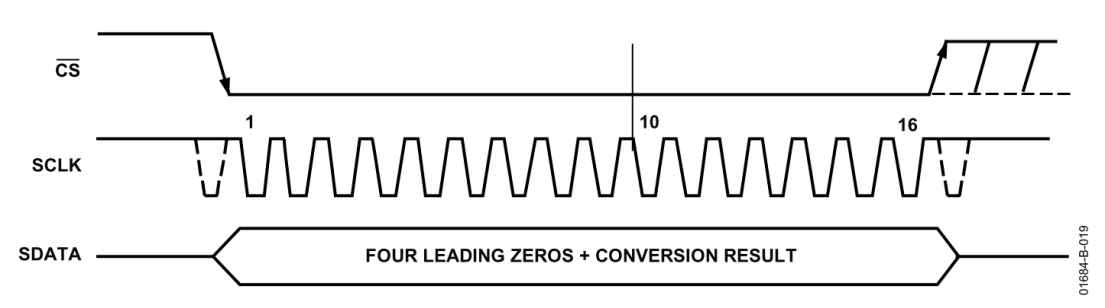
\includegraphics[width=0.7\linewidth]{images/adc}
	\caption{Использованный в приборе ДЭПРОН режим работы АЦП (AD7495), по материалам:  «1 MSPS,12-Bit ADCs  AD7475/AD7495», One Technology Way, P.O. Box 9106, Norwood, MA 02062-9106, U.S.A., 2005 Analog Devices, Inc.}
	\label{fig:adc}
\end{figure}

В первой версии платы цифровой обработки сигналов подключение обоих АЦП к контроллеру прибора производилось по независимым каналам: CS (Chip Select -- Активный логический вход АЦП), SCLK (Serial Clock -- логический вход АЦП), SDATA (Data Output -- логический выход АЦП). Задача максимально быстрого захвата сигналов с выхода предусилителя решалась включением встроенного в АЦП устройства выборки и хранения (англ. ``track and hold circuit'') в момент получения контроллером сигнала от таймингового выхода предусилителя. Для этого прерывания контроллера настроены при получении такого сигнала на выдачу управляющего сигнала на вход CS АЦП, ответственного за оцифровку сработавшего канала аналоговой части прибора. Дальнейшая оцифровка амплитуды захваченного в буфере АЦП сигнала производилась после выхода из процедуры обработки прерывания, так как этот процесс отнимает значительное время. Испытания процедуры управления оцифровкой АЦП показали, что точность измерений АЦП чувствительна к временной регулярности тактирующего сигнала подаваемого на SCLK АЦП. Одной из причин таких нерегулярностей является возможность срабатывания прерывания в ПО контроллера во время исполнения процедуры генерации тактирующих импульсов, что в условиях эксплуатации прибора при высоких потоках ионизирующих излучений (например, в области ЮАА) не редкость. Временное отключение обработки прерываний может устранить данный недостаток работы прибора, однако испытания такого режима работа показали накопление необработанных прерываний в буфере контроллера, которые впоследствии обрабатывались неверно, из-за чего решено отказаться от использования этого режима.


\todo{Рисунок. Осциллограмма: регулярность тактирующего сигнала, подающегося на SCLK АЦП.}

Выявление нерегулярности тактирующего сигнала потребовало проверку этого сигнала с помощью осциллографа. Дизассемблирование скомпилированного кода ПО микроконтроллера показало критические места кода, требующие изменения алгоритма генерации тактирующих импульсов и добавления промежутков простоя процессора (\texttt{\_nop} -- в коде ``no operation''). Окончательная проверка регулярности сигнала, генерируемого выверенным кодом, производилась снятием временной развертки тактирующего сигнала  на осциллографе. Данный подход использовался и при последующих отработках работы АЦП прибора ДЭПРОН.

\todo{Рисунок Блок схема подключения АЦП к контроллеру версия 1.}

Таким образом, в первой версии платы цифровой обработки сигналов использовались шесть независимых каналов контроллера, что ограничивало возможность подключения дополнительных информационных каналов с детекторной части прибора. Также одой из проблем данного подхода является двойная нагрузка на микроконтроллер прибора ДЭПРОН, так как управляющие сигналы генерируются программным способом. Такой подход предоставлял сомнительное преимущество в независимом управлении АЦП из программного обеспечения микроконтроллера, поэтому было принято решение изменения способа подключения АЦП.

Следующим конструктивным решением было включение обоих АЦП в параллельный режим работы, когда управляющий (CS) и тактирующий (SCLK) сигналы подаются на оба АЦП. Каналы данных (SDATA) подключены к независимым входам контроллера. 

\todo{Рисунок Блок схема подключения АЦП к контроллеру версия 2.}

При проектировании Блоков обработки Информации (БИ) было принято решение по организации обмена по каналу CAN между дочерними приборами, входящими в Комплекс Научной Аппаратуры (КНА) «Ломоносов». Однако использованный для макетирования контроллер ATmega128, и данный контроллер был заменен на AT90CAN128. Данное решение было продиктовано минимальными изменениями уже разработанного программного обеспечения и незначительными доработками печатных плат, необходимым для внедрения контроллера AT90CAN128.

Опыт работы с данным контроллером также показал его применимость для целей построения полноценного дозиметра ионизирующих излучений. Тем не менее, по требованию других участников проекта данный контроллер был заменен более современным и более производительным контроллером AT91SAM7X256. Всего в составе КНА насчитывается 4 прибора, в которых использована схема цифровой обработки сигнала на базе AT91SAM7X, некоторые из этих приборов испытывали нехватку производительности данного модуля до замены ЦПУ. В целях унификации разработанный аппаратуры модуль цифровой обработки сигналов и связи был заменен и в приборе ДЭПРОН. Данное изменение состава прибора повлекло за собой необходимость повторения цикла разработки программно-математического обеспечения прибора и проведения повторных калибровок АЦП и счетных каналов схемы цифровой обработки. Необходимость данных работ обусловлена принципиальным отличием архитектуры контроллера: в исходном варианте это архитектура AVR, а в окончательном ARM. 

В финальном варианте цифровая обработка сигналов осуществляется с помощью микропроцессора AT91SAM7X512. Программно-математическое обеспечение ДЭПРОН функционирует на одной микропроцессорной плате SSD234. Данная плата собрана на базе микроконтроллера AT91SAM7X512 производства фирмы ATMEL, и содержит процессор ARM7 TDMI® ARM® Thumb® с 32-разрядной RISC-архитектурой команд.

Программное обеспечение процессора осуществляет регистрацию сигналов, поступающих со схем преобразования импульсов с детекторов, их преобразование и накопление, передачу результатов по каналу связи с блоком информации КА. Объем сбрасываемой информации не превышает 1 Мбайт/сутки.

\section{Связь с внешними системами}
\emph{Связь с Блоком Информации «Ломоносов»}

Связь с БИ осуществляется посредством канала Controller Area Network (CAN), использующегося в качестве стандарта промышленных сетей. CAN ориентированн на объединение в единую сеть различных исполнительных устройств и датчиков. Режим передачи данных - последовательный, широковещательный, пакетный. Программные модули и аппаратные схемы разрабатывались для комплекса аппаратуры в целом Н.Н. Веденькиным и прошли проверку при доводке аппаратуры и комплексных испытаниях КНА.

Прибор ДЭПРОН формирует в рабочем режиме пакеты данных по 512 байт, которые накапливаются во внутренней памяти контроллера. Подготовленная очередь пакетов  передается на БИ КА «Ломоносов», где накапливается для передачи на Землю.

Передача информации от космического аппарата происходит через сеть фиксированной спутниковой связи. Данные передаются через общественную сеть Интернет и архивируются на специально выделенном сервере данных. Альтернативно, при отсутствии подключения к спутниковой сети связи, используется канал передачи телеметрической информации с платформы КА «Ломоносов», при таком подключении данные ДЭПРОН поступают на Землю через центр управления полетами (ЦУП) и ввиду ограниченной пропускной способности этого канала данные передаются частично.

\emph{Связь с прибором ИМИСС}

Связь с прибором ИМИСС-1 осуществляется по каналу RS232 (USART). Поступающая информация транслируется прибором ДЭПРОН в БИ по каналу CAN без изменений. В соответствии с расчетным объемом данных от прибора ИМИСС затраты производительности микроконтроллера ДЭПРОН на трансляцию данных в БИ будут незначительны по отношению к затратам на выполнение основных задач прибора ДЭПРОН.

\subsection{Питание}

Электропитание схем прибора ДЭПРОН осуществляется с использованием DC/DC преобразователей. Напряжение питание бортовой сети 27В, подключено через разъем Х2 прибора ДЭПРОН и поступает на два преобразователя 28/12 В. С первого преобразователя напряжение поступает на стабилизатор напряжения и далее из этого напряжения формируются номиналы: +6 В, для питания схем усилителей, формирователей и микропроцессора. Со второго преобразователя питание поступает на преобразователь +70 В, для питания полупроводниковых детекторов и на преобразователь +1200 В, для питания газоразрядных счетчиков. 

\subsection{Программное обеспечение}

Программно-математическое обеспечение прибора ДЭПРОН состоит из программы для контроллера прибора, написанной на языке C++(C), c использованием пакета IAR  Workbench\textsuperscript{®} для микроконтроллеров архитектуры ARM\textsuperscript{®}. 


Исполняемый код программы формируется из двух файлов: 


\begin{itemize}
	\item 	\texttt{detector.c} -- прикладные функции для работы прибора ДЭПРОН
	
	
	\item \texttt{main.cpp} -- инициализация контроллера прибора и функции обмена информацией с БИ. В процедуре main этого файла работает основной бесконечный цикл программы, в котором вызываются функции обмена информацией по каналу CAN и процедура \texttt{Detectors\_Handling}.
	
	
\end{itemize}
Работа прибора ДЭПРОН основана на прерываниях, которые обрабатываются по мере их поступления в процедуре \texttt{Ext\_Interrupt} (см. рисунок \ref{fig:ext_interrupt}), а ресурсоемкий разбор полученных данных и запуск АЦП происходят в процедуре \texttt{Detectors\_Handling}, которая отрабатывает постоянно. 

\begin{figure}
\centering
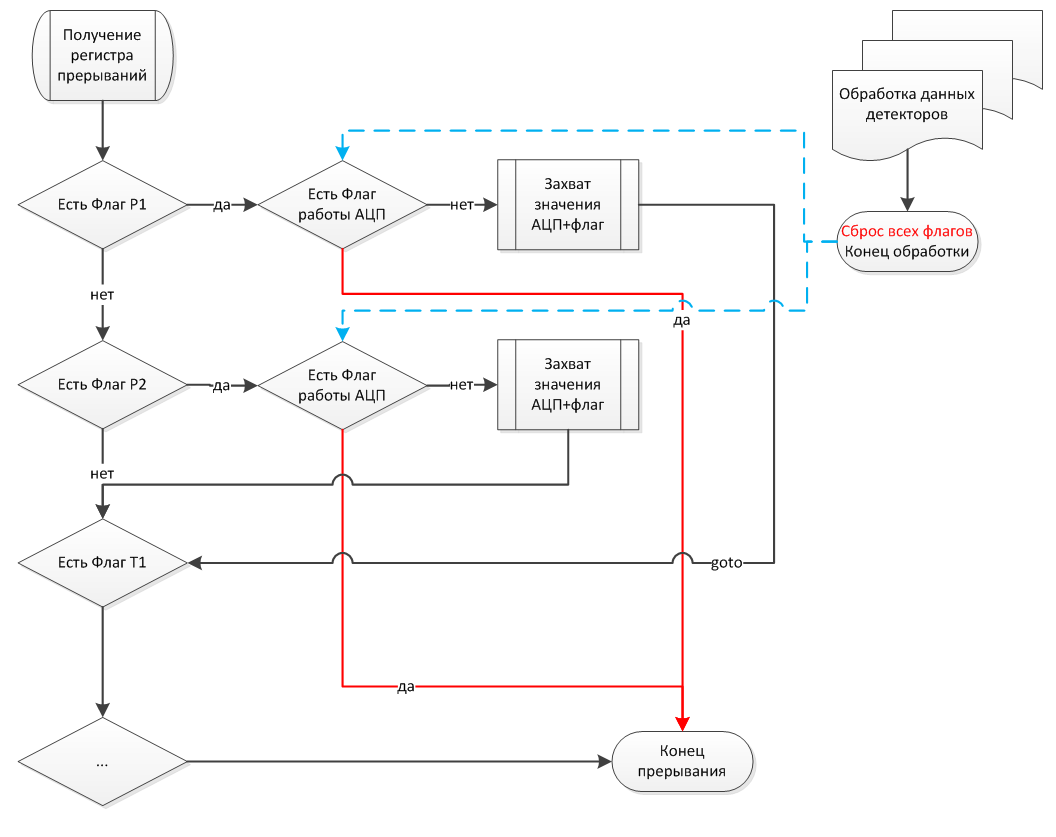
\includegraphics[width=0.7\linewidth]{images/ext_interrupt}
\caption{Блок схема работы процедуры \texttt{Ext\_Interrupt}, \todo{требует обновления!}}
\label{fig:ext_interrupt}
\end{figure}


\todo{Таблица Распределение битов в регистре прерывания}


\subsubsection{Процедура обработки данных с детекторов}
{\small 
\begin{verbatim}
void Detectors_Handling(void)
{  
	//int i; char* p1; // char* p2;
	int J, K;
	if (!Detectors_Flugs) {
		long interrupt_register = AT91C_BASE_PIOB->PIO_ISR;    
		return;
	}  
	Temporal_buff.FLUGS = Detectors_Flugs;
	// Prot_Comp_1++;    //__________________________ !!! FOR debuging !!! ________________
	if (Detectors_Flugs & Detec_Flug_ADC){
		dataADC = External_ADC_Read_Double();
		Temporal_buff.ADC_code = dataADC;
	} else dataADC = 0;
	
	
	if (Detectors_Flugs & Detec_Flug_compar){
		Prot_Comp_1++;  Prot_Comp_2++;  
		J= (((dataADC+3)>>3) & 0X00000FFF);
		Dose_Comp_1+=J;
		K= Digital_Compression(J);
		if (K<2) K=2; if(K>63) K=63;
		Spectra[2][K]++;
		
		//  ADC_code_2=dataADC+0x00030000;
		
		J= (((dataADC+0x00030000)>>19) & 0X00000FFF);   //(short )
		Dose_Comp_2+=J;
		K= Digital_Compression(J);
		if (K<2) K=2; if(K>63) K=63;
		Spectra[3][K]++;
		
	} else {
	if ((Detectors_Flugs & Detec_Flug_P1)&&( dataADC & 0X00003FF0)){
		J= (((dataADC+3)>>3) & 0X00000FFF);
		Dose_1+=J;  Prot_1++;
		K= Digital_Compression(J);
		if (K<2) K=2; if(K>63) K=63;
		Spectra[0][K]++;
	}
	if ((Detectors_Flugs & Detec_Flug_P2)&&( dataADC & 0X3FF00000)){
		J= (((dataADC+0x00030000)>>19) & 0X00000FFF);
		Dose_2+=J;  Prot_2++;
		
		K= Digital_Compression(J);
		if (K<2) K=2; if(K>63) K=63;
		Spectra[1][K]++;
		
	}
}
if (Detectors_Flugs & Detec_Flug_N1){      
	Neutron_1 += Neut_1;
	Neut_1 = 0;
} 

if (Detectors_Flugs & Detec_Flug_N2){       
	Neutron_2 += Neut_2; 
	Neut_2 = 0;
} 

if(Temporal_buff.interr_reg & Detector_Interrupt_t1) {
	if(High_Ampl_Buffer.ind==0){
		High_Ampl_Buffer.day[0]= t_info.day;
		High_Ampl_Buffer.day[1]= t_info.Mounth;
	}    
	High_Ampl_Buffer.HA[High_Ampl_Buffer.ind].ADC_code = dataADC;
	High_Ampl_Buffer.HA[High_Ampl_Buffer.ind].ta[0] = tick_1;
	High_Ampl_Buffer.HA[High_Ampl_Buffer.ind].ta[1] = t_info.secunde;
	High_Ampl_Buffer.HA[High_Ampl_Buffer.ind].ta[2] = t_info.minute;
	High_Ampl_Buffer.HA[High_Ampl_Buffer.ind].ta[3] = t_info.hour;
	High_Ampl_Buffer.ind++;
	if(High_Ampl_Buffer.ind>62) Send_High_Ampl_Buffer();    
}     
//For Neutron burst 
unsigned long N_T;
unsigned short millisec_time = AT91C_BASE_TC2->TC_CV;
millisec_time = millisec_time >>3;   //40 kHz / 8 = 5 kHz
if ((Pronon_Fon < Proton_Level) && (N_ind > 0) && (Detectors_Flugs & Detec_Flug_Neutron)){      
	if (((millisec_time - Old_Tick_2)< D_tick_2) && (Old_Sec== t_info.day_second)){
		N_T= t_info.day_second <<15;
		N_T |= Old_Tick_2 & 0x00001fff;
		if (Detectors_Flugs & Detec_Flug_N1) N_T |= 0x00002000;
		if (Detectors_Flugs & Detec_Flug_N2) N_T |= 0x00004000;
		Neutron_Bunch.neutron_t[i_n_t++]=N_T;
		if(i_n_t>126) Send_Neutron_Bunch();
	}
}
Old_Sec = t_info.day_second;
Old_Tick_2 = millisec_time;        


Detectors_Flugs=0;

}  
\end{verbatim}
}

\todo{Блок схема работы процедуры Detectors\_Handling}

{\small 
\begin{verbatim}
// Test conversion program
	
#include <iostream>
#include <string>

int main()
{
	std::string name;
	//getline (std::cin, name);
	unsigned short dataADC, J, K, L;
	dataADC = 114;
	
	std::cout << "Was " << dataADC << "!\n";
	
	J= (((dataADC+3)>>3) & 0X00000FFF);
	
	std::cout << "Present " << J << "!\n";
	K= (J<<3);
	std::cout << "Left shift " << K << "!\n";
	L= (J*8);
	std::cout << "Multyply*8 " << L << "!\n";
}
\end{verbatim}
}



\subsection{Контрольная проверочная аппаратура}

Контрольно приемная аппаратура (КПА) прибора ДЭПРОН используется для  проведения автономных испытаний прибора. КПА ДЭПРОН состоит из:


\begin{itemize}
	\item 	Ноутбук (или другой персональный компьютер) с установленной операционной системой Windows XP и установленным специальным программным обеспечением (программой Depron Terminal), наличием порта RS232, либо дополнительно преобразователь интерфейсов USBRS232;
	
	
	\item 	Блока питания, обеспечивающего измерение потребляемого тока нагрузки GwINSTEK GPS-4303;
	
	
	\item 	Преобразователя интерфейсов USBRS232 (при отсутствии COM порта у ПК);
	
	
	\item 	Комплекта соединительных кабелей 
	
	
	\item 	Блока КП -- контрольно-приемного блока
	
	
\end{itemize}






\todo{Рис.1. Схема подключения КПА для проверки функционирования прибора ДЭПРОН.}


Блок КП предназначен для подключения генератора и осциллографа к тестовым входам прибора ДЭПРОН, а также для контроля наличия рабочих напряжений в контурах прибора. Блок КП имеет 4 входных гнезда BNC промаркированных в соответствии с каналами прибора ДЭПРОН на которые передаются тестовые сигналы с генератора: 



\begin{itemize}
	
	\item 	X1	
	
	\item 	X2\ldots
		
\end{itemize}

На лицевой панели блока КП расположены 2 светодиодных индикатора. Подключение Блока КП к прибору ДЭПРОН происходит через тестовый вход XT3 (типа РС19).


\section{Градуировочные  характеристики прибора}
Градуировка прибора ДЭПРОН проводится с использованием известной зависимости 
\ref{eq:benghin_doze_code}

\begin{equation}\label{eq:benghin_doze_code}
D = \frac{E}{m} = \dfrac{w_i \cdot\frac{q}{e}}{m} = \frac{w_i \cdot \Delta U \cdot\sum K \cdot C}{m \cdot e \cdot \eta}  = V \cdot \sum K
\end{equation}
по материалам  «ПРИБОР ДЭПРОН, В.В. Бенгин, О.Ю. Нечаев, И.А. Брильков, А. Амелюшкин, В. Петров»  представленной на рабочем совещании «Universat» (Университетские спутники), 7-10 июня в МГУ им. М.В. Ломоносова

где \begin{description}	
	\item[$ K $] выходной сигнал АЦП
	\item[$ C $] входная емкость системы детектор-предусилитель
	\item[$ \eta $] суммарный градуировочный коэффициент тракта усиления до АЦП
	\item[$ \Delta U $] шаг дискретизации АЦП
\end{description} 
Большая часть величин в этой формуле известна, а экспериментально были определены недостающие величины. Данная работа была проведена Сиолаповым Виктором под руководством Бенгина В.В., опираясь на полученные результаты можно провести расчет энергетических коэффициентов для получения величин дозы.

Детектор1: 3,4141 КэВ/канал 

Детектор2: 4 КэВ/канал - очень большой разброс по калибровкам - не могу понять почему:15.4 – 16.3 КэВ/канал. Необходимо найти исходные данные калибровок.

В ходе калибровок получено, что одной еденице по дозе детектора 1 соответствует 135 счетных имульсов в детектору 1, получается что умножив 135 на 3,4141  КэВ/канал  получаем энергетический эквивалент 3687 КэВ/(дозовый импульс) 

Так как мы имеем квадратный детектор с размерами 10мм * 10мм* 300мкм, оценим массу чувствительного объема детектора, подборав значения толщины тормозящего слоя вещества $ 0.0013 $ г/см$^2 $. Такая масса соответствует 5,58 мкм кремния или 1,04 см воздуха, а масса детектора соответственно: 0,0687г.

Дет1: 8,69пГр/кодАЦП  0,06952 = наноГрей/импульс(умноженное на 8)

Дет2: 9,32пГр/кодАЦП  0,07456 = наноГрей/импульс(умноженное на 8)


В программе микроконтроллера Дэпрон с целью сокращения передачи неинформативных 
каналов АЦП был сделан сдвиг на 3 разряда при записи в спектр энерговыделения, 
такая операция близка к операции деления на 8.

Независимый расчет дал результат для коэффициентов для первого детектора 
0,0633  наноГрей/импульс, для второго -  0,0742 наноГрей/импульс. С учетом 
коэффициента 8 это близко к полученным результатам.

\section{Энергетическая чувствительность прибора ДЭПРОН}

В процессе разработки прибор не проходил в полном объеме испытаний на 
спектральную чувствительность к различным типа излучений, были проведены только 
калибровки детектирующих узлов на радиоактивных источниках. 

По соображениям Бенгина В.В. наиболее чувствительный параметр --- скорость 
счета 
детектора 1. Так как детектор закрыт сверху алюминиевой крышкой толщиной 2 мм, 
он должен быть чувствителен к протонам с энергией больше 20 МэВ и электронам с 
энергией больше примерно 0,5 МэВ, а также - возможно - к тормозному излучению. 
Порог дискриминации сигналов с детектора около 100 КэВ.
Тем не менее вопрос уточнения границы чувствительности по минимальным энергиям 
продолжает оставаться важным и на первом этапе были проведены оценки с помошью 
данных  по проникновению электронов и протонов с сайта NIST \cite{NIST}, 
физическая модель  лежащая в основе этих данных основывается на теории 
Бете\cite{Bethe1930} с поправкой Штернхаймера \cite{Sternheimer1952} на 
плотность вещества  и подробно описана в 
ряде статей этого института \cite{Bichsel1992,Ashley1972}.

\begin{figure}[H]
	\centering
	\fcolorbox{red}{yellow}{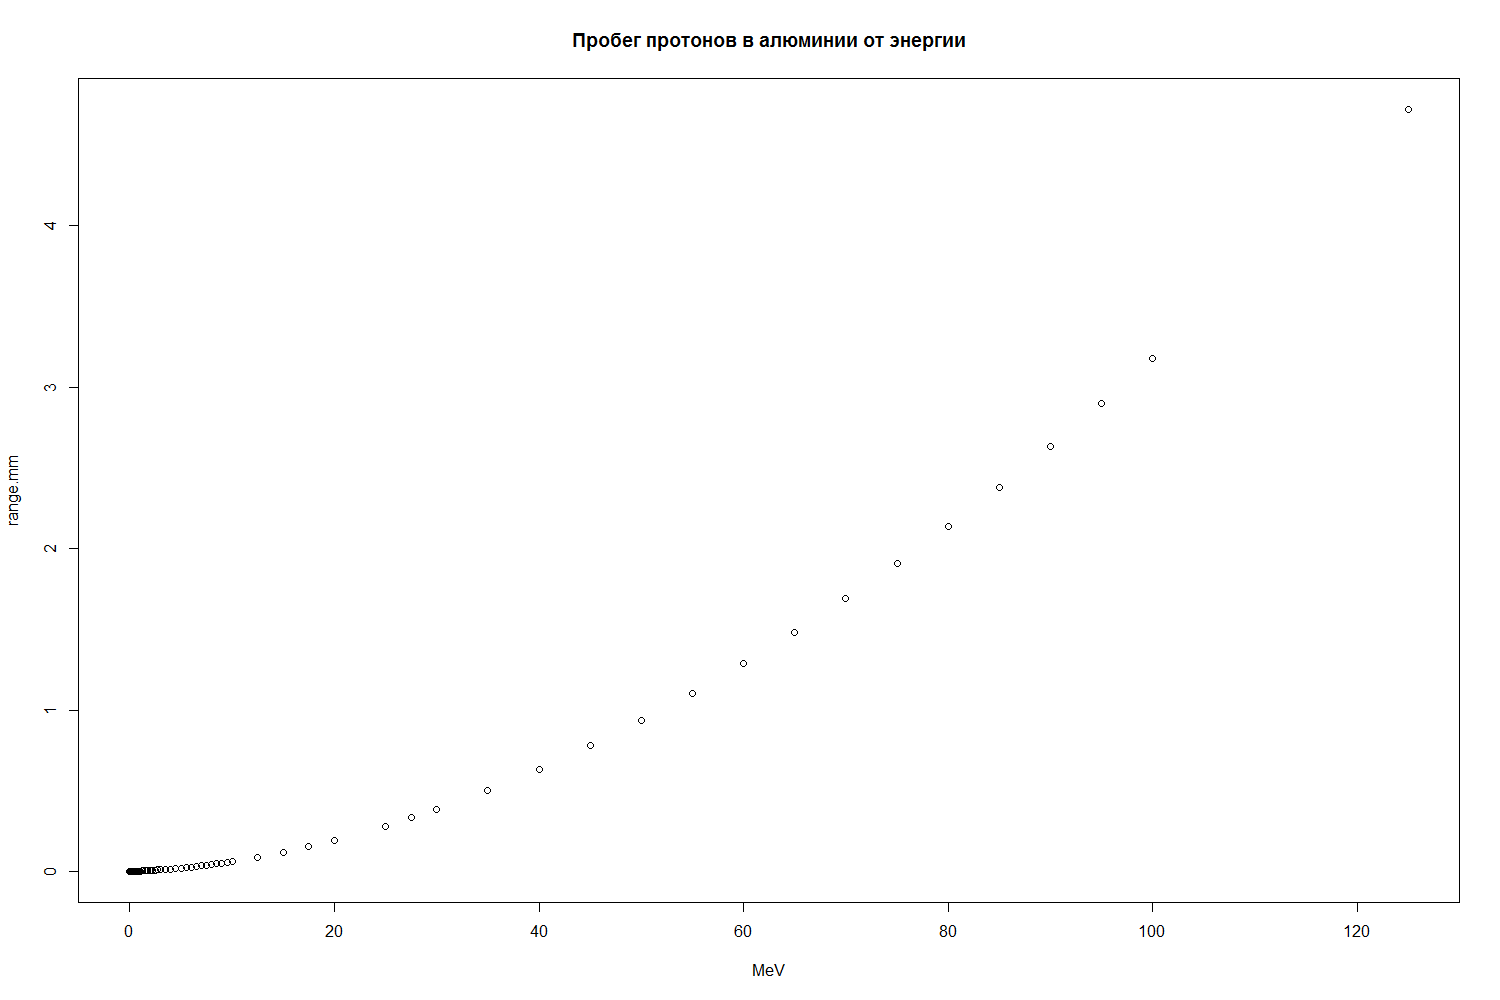
\includegraphics[width=0.6\linewidth]{images/Rplot01}
	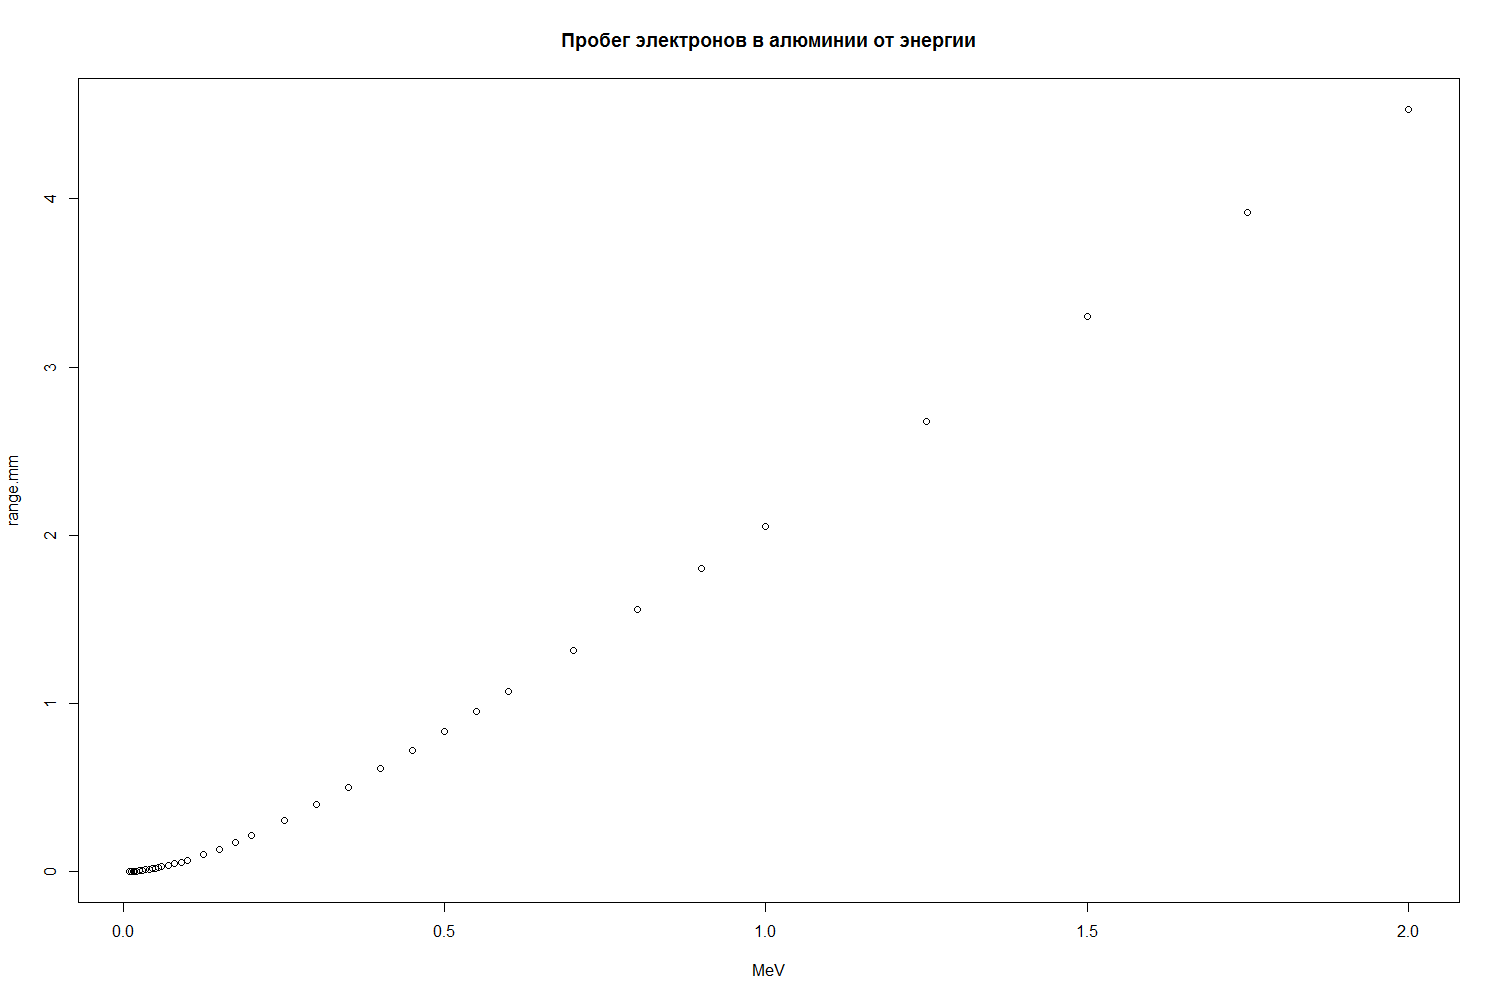
\includegraphics[width=0.6\linewidth]{images/Rplot02}}
	\caption{Графики средних пробегов заряженных частиц для алюминия. 
	Представлены величины: ``CSDA range'' --- глубина в приближении 
	непрерывного замедления
	``Projected range'' --- среднее значение глубины, на которую заряженная 
	частица проникает в процессе замедления до остановки}
	\label{fig:rplot01}
\end{figure}

\begin{figure}
	\centering
	\fcolorbox{red}{yellow}{
		{\color{green}
		\stackinset{l}{1in}{b}{1.1in}{\rotatebox{0}{\rule{3.5in}{1pt}}}{%
			\stackinset{l}{.3in}{b}{}{\rotatebox{85}{\rule{4in}{1pt}}}{%
				\stackinset{r}{.5in}{b}{}{\rotatebox{-80}{\rule{4in}{1pt}}}{%
					\stackinset{r}{1in}{b}{-.3in}{\rotatebox{-85}{\rule{4in}{1pt}}}{%
						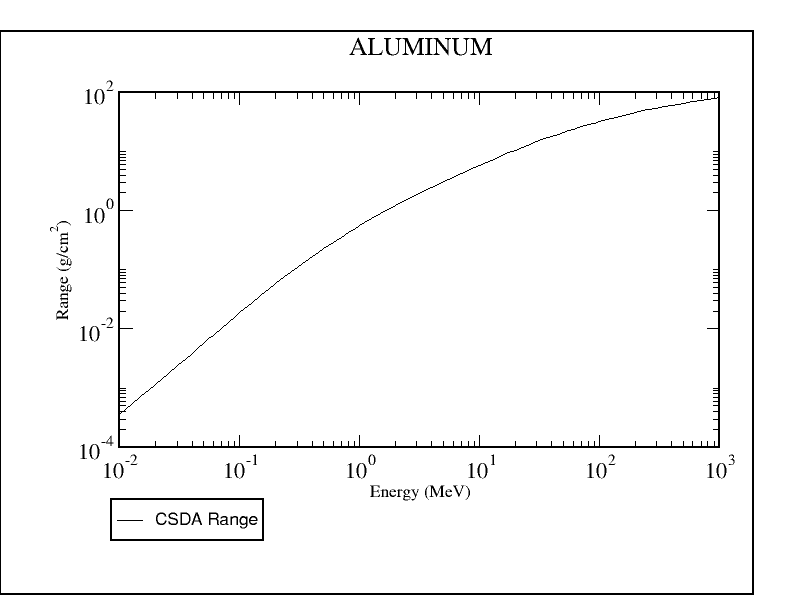
\includegraphics[width=3.5in]{images/graph_elec}
						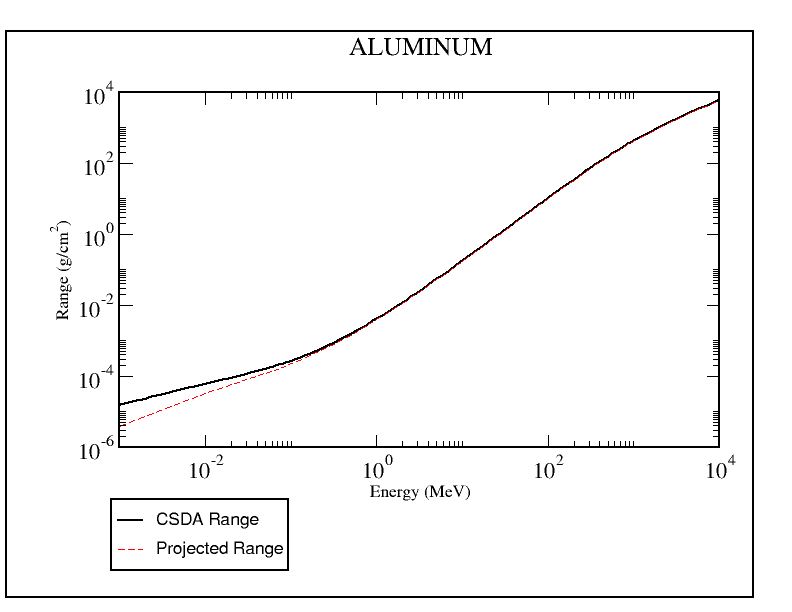
\includegraphics[width=3.5in]{images/graph_prot}
						%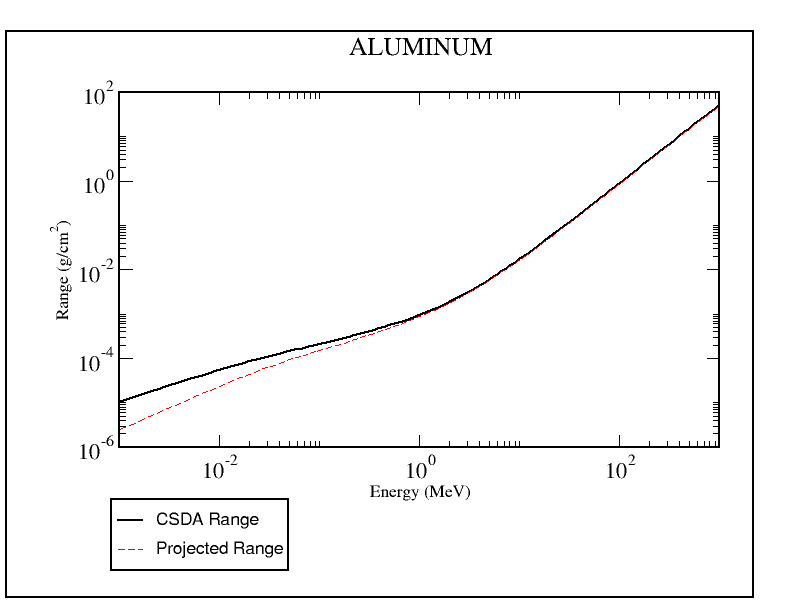
\includegraphics[width=0.7\linewidth]{images/graph_alpha}%
	}}}}}}
	\caption{}
\label{fig:graphelec}
\end{figure}

Пользуясь представленными зависимостями, для уточненной минимальной толщины 
корпуса прибора --- она составляет 2,5 мм, что составляет 0,65 
г/см\textsuperscript{2}, была 
повышена предварительная 
оценка  
порога нижних энергий которые способен регистрировать Дэпрон по электронам до 1 
МэВ и по протонам до 80 МэВ. Так как эти зависимости могут использоваться 
только для средних пробегов частиц, для оценки функции энергетической 
чувствительности требуется более подробный анализ, который может быть 
произведен с помошью Монте-Карло моделирования.

